% ╔══════════════════════════════════════════════════════════════╗
% ║  Process Engineer Interview Presentation — Chang Ho Yu       ║
% ║  Style: sea_turtle_blood_detection_presentation (Beamer)     ║
% ║  Compile: xelatex interview-slides.tex  (twice)              ║
% ╚══════════════════════════════════════════════════════════════╝

\documentclass[aspectratio=169,10pt]{beamer}

% ─── Fonts ─────────────────────────────────────────────────────
\usepackage{fontspec}
\usepackage{xeCJK}
\setCJKmainfont{Microsoft JhengHei}
\setCJKsansfont{Microsoft JhengHei}
\setmainfont{Calibri}
\setsansfont{Calibri}

% ─── Packages ──────────────────────────────────────────────────
\usepackage{graphicx}
\usepackage{booktabs}
\usepackage{tikz}
\usepackage{xcolor}
\usepackage{array}
\usepackage{colortbl}
\usepackage{amssymb}
\usetikzlibrary{arrows.meta,positioning,shapes.misc}

% ─── Colors ────────────────────────────────────────────────────
\definecolor{mainblue}{RGB}{55,55,155}
\definecolor{lightblue}{RGB}{220,222,248}
\definecolor{alertred}{RGB}{160,20,20}
\definecolor{alertpink}{RGB}{252,222,222}
\definecolor{successgreen}{RGB}{25,110,50}
\definecolor{lightgreen}{RGB}{210,240,218}

% ─── Theme ─────────────────────────────────────────────────────
\usetheme{default}
\usecolortheme[named=mainblue]{structure}

\setbeamercolor{title}{fg=white, bg=mainblue}
\setbeamercolor{frametitle}{fg=mainblue, bg=white}
\setbeamercolor{block title}{fg=white, bg=mainblue}
\setbeamercolor{block body}{fg=black, bg=lightblue!45}
\setbeamercolor{block title alerted}{fg=white, bg=alertred}
\setbeamercolor{block body alerted}{fg=black, bg=alertpink}
\setbeamercolor{block title example}{fg=white, bg=successgreen}
\setbeamercolor{block body example}{fg=black, bg=lightgreen}
\setbeamercolor{itemize item}{fg=mainblue}
\setbeamercolor{itemize subitem}{fg=mainblue}
\setbeamercolor{author in head/foot}{fg=white, bg=mainblue!90}
\setbeamercolor{title in head/foot}{fg=white,  bg=mainblue!70}
\setbeamercolor{date in head/foot}{fg=white,  bg=mainblue!90}

% ─── Footer ────────────────────────────────────────────────────
\setbeamertemplate{footline}{
  \leavevmode
  \hbox{%
    \begin{beamercolorbox}[wd=.333\paperwidth,ht=2.4ex,dp=1.2ex,left]
      {author in head/foot}
      \hspace{1.2em}\usebeamerfont{author in head/foot}\insertshortauthor
    \end{beamercolorbox}%
    \begin{beamercolorbox}[wd=.334\paperwidth,ht=2.4ex,dp=1.2ex,center]
      {title in head/foot}
      \usebeamerfont{title in head/foot}\insertshorttitle
    \end{beamercolorbox}%
    \begin{beamercolorbox}[wd=.333\paperwidth,ht=2.4ex,dp=1.2ex,right]
      {date in head/foot}
      \usebeamerfont{date in head/foot}\insertshortdate{}\hspace{2em}
      \insertframenumber{} / \inserttotalframenumber\hspace{1.2em}
    \end{beamercolorbox}}%
  \vskip0pt%
}
\setbeamertemplate{navigation symbols}{}
\setbeamertemplate{itemize item}{\small\textbullet}
\setbeamertemplate{itemize subitem}{\small\textbullet}
\setbeamerfont{frametitle}{size=\large,series=\bfseries}

% ─── Meta ──────────────────────────────────────────────────────
\title[Process Engineer Interview]{Process Engineer Interview Presentation}
\subtitle{Semiconductor Manufacturing}
\author[Chang Ho Yu]{Chang Ho Yu \quad 張合羽}
\institute{M.S. Biological Sciences, National Taiwan University}
\date{April 2026}

% ═══════════════════════════════════════════════════════════════
\begin{document}

% ── Slide 1: Title ─────────────────────────────────────────────
\begin{frame}
  \titlepage
\end{frame}

% ── Slide 2: Outline ───────────────────────────────────────────
\begin{frame}{Outline}
  \tableofcontents
\end{frame}

% ═══════════════════════════════════════════════════════════════
\section{About Me}
% ── Slide 3: About Me ──────────────────────────────────────────
\begin{frame}{About Me}
  \begin{columns}[T]
    \column{0.50\textwidth}
      \begin{block}{Education}
        \small
        \begin{itemize}
          \item \textbf{M.S.} National Taiwan University\\
                Ecology \& Evolutionary Biology\\
                {\footnotesize 2023--2025 \quad GPA 4.0\,/\,4.3}
          \item \textbf{B.S.} National Cheng Kung University\\
                Department of Life Sciences\\
                {\footnotesize 2019--2023}
        \end{itemize}
      \end{block}
      \vspace{0.1cm}
      \begin{block}{Awards}
        \small
        \begin{itemize}
          \item $\bigstar$\ \textbf{Top Honor} — NTU IEEB Student\\
                Academic Presentation Competition, 2025
          \item NSTC Undergraduate Research Grant
        \end{itemize}
      \end{block}

    \column{0.46\textwidth}
      \begin{block}{Core Strengths}
        \small
        \begin{itemize}
          \item \textbf{DOE / Taguchi Method}\\
                {\footnotesize 6-parameter simultaneous optimization}
          \item \textbf{SOP Development from Scratch}\\
                {\footnotesize Full validation, zero prior reference}
          \item \textbf{Root-Cause Analysis (RCA)}\\
                {\footnotesize 5-Why, fishbone, CAPA}
          \item \textbf{Automated QC Pipeline}\\
                {\footnotesize QuPath scripting, +70\% throughput}
          \item \textbf{Statistical Analysis (SAS)}\\
                {\footnotesize Multi-variable comparison}
        \end{itemize}
      \end{block}
  \end{columns}
\end{frame}

% ═══════════════════════════════════════════════════════════════
\section{Core Technical Skills}
% ── Slide 4: Skills ────────────────────────────────────────────
\begin{frame}{Core Technical Skills}
  \begin{columns}[T]
    \column{0.48\textwidth}
      \begin{block}{Process Engineering}
        \small
        \begin{itemize}
          \item DOE / Factorial Design (Taguchi Method)
          \item SOP development and process validation
          \item Batch QC and acceptance criteria setting
          \item RCA (root-cause analysis) and CAPA
        \end{itemize}
      \end{block}
      \vspace{0.1cm}
      \begin{block}{Data \& Automation}
        \small
        \begin{itemize}
          \item SAS statistical analysis
          \item QuPath scripting (automated QC pipeline)
          \item AI segmentation model fine-tuning
        \end{itemize}
      \end{block}

    \column{0.48\textwidth}
      \begin{block}{Laboratory Techniques}
        \small
        \begin{itemize}
          \item IHC / IF immunofluorescence staining
          \item Western Blot \& qPCR
          \item Cryosectioning \& primary cell culture
          \item LAC / NHRI laboratory certifications
        \end{itemize}
      \end{block}
      \vspace{0.1cm}
      \begin{block}{Cross-functional Coordination}
        \small
        \begin{itemize}
          \item 100+ member, 5-institution field operations
          \item Teaching assistant (30+ laboratory sessions)
          \item Scientific presentation in English
        \end{itemize}
      \end{block}
  \end{columns}
\end{frame}

% ═══════════════════════════════════════════════════════════════
\section{M.S. Research: Process Development}
% ── Slide 5: Graduate Research ─────────────────────────────────
\begin{frame}{M.S. Research: SOP from Scratch}
  \begin{block}{Background}
    \small
    Histological analysis of cetacean skin (\textit{Lagenodelphis hosei}) ---
    \textbf{no existing protocol}; complete 6-module process built independently.
  \end{block}

  \vspace{0.1cm}
  \begin{center}
  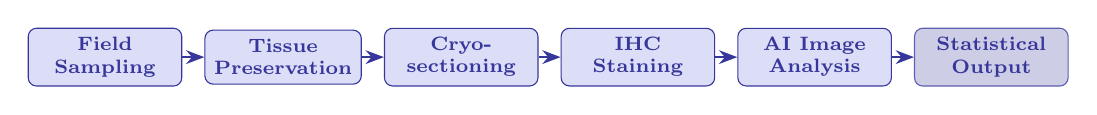
\begin{tikzpicture}[
    snode/.style={draw=mainblue, fill=lightblue, rounded corners=3pt,
                  minimum width=1.95cm, minimum height=0.52cm,
                  font=\scriptsize\bfseries\color{mainblue}, align=center},
    arr/.style={-Stealth, thick, mainblue}
  ]
    \node[snode] (s1) {Field\\Sampling};
    \node[snode, right=0.28cm of s1] (s2) {Tissue\\Preservation};
    \node[snode, right=0.28cm of s2] (s3) {Cryo-\\sectioning};
    \node[snode, right=0.28cm of s3] (s4) {IHC\\Staining};
    \node[snode, right=0.28cm of s4] (s5) {AI Image\\Analysis};
    \node[snode, fill=mainblue!25, draw=mainblue!80,
          right=0.28cm of s5] (s6) {Statistical\\Output};
    \foreach \a/\b in {s1/s2,s2/s3,s3/s4,s4/s5,s5/s6}
      \draw[arr] (\a) -- (\b);
  \end{tikzpicture}
  \end{center}

  \vspace{0.1cm}
  \begin{columns}[T]
    \column{0.50\textwidth}
      \begin{block}{Challenge $\rightarrow$ Skill Gained}
        \footnotesize
        \begin{tabular}{p{2.8cm}p{2.4cm}}
          \toprule
          Challenge & Skill Gained \\
          \midrule
          No existing protocol  & SOP from scratch \\
          High variability      & Batch QC mgmt. \\
          6-param. tuning       & DOE mindset \\
          5-institution team    & Cross-func. coord. \\
          \bottomrule
        \end{tabular}
      \end{block}

    \column{0.46\textwidth}
      \begin{alertblock}{Quantified Results}
        \small
        \begin{itemize}
          \item Throughput \textbf{increased by +70\%}
          \item Segmentation accuracy \textbf{92\% $\to$ 99\%}
          \item 5 institutions adopted the SOP
          \item Zero repeat batch failures after CAPA
        \end{itemize}
      \end{alertblock}
  \end{columns}
\end{frame}

% ═══════════════════════════════════════════════════════════════
\section{DOE Taguchi Optimization}
% ── Slide 6: DOE ───────────────────────────────────────────────
\begin{frame}{DOE Taguchi Method: 6-Parameter Optimization}
  \begin{columns}[T]
    \column{0.50\textwidth}
      \begin{block}{Six Process Parameters}
        \footnotesize
        \begin{tabular}{@{}cl@{}}
          \toprule
          \# & Parameter \\
          \midrule
          P1 & Antibody Concentration \\
          P2 & Incubation Time \\
          P3 & Antigen Retrieval Temperature \\
          P4 & Retrieval Duration \\
          P5 & Blocking Agent Concentration \\
          P6 & Section Thickness \\
          \bottomrule
        \end{tabular}
      \end{block}
      \vspace{0.1cm}
      \begin{block}{Experimental Efficiency}
        \small
        \begin{itemize}
          \item Full factorial: $3^{6} = 729$ runs required
          \item Taguchi $L_{18}$ orthogonal array: \textbf{18 runs}
          \item \textbf{97.5\% reduction} in experiment count
        \end{itemize}
      \end{block}

    \column{0.46\textwidth}
      \begin{block}{Analysis Approach}
        \small
        \begin{itemize}
          \item Signal-to-Noise (S/N) ratio analysis
          \item Main effect ranking per factor
          \item Optimal level combination selection
          \item Confirmation run validation
        \end{itemize}
      \end{block}
      \vspace{0.1cm}
      \begin{alertblock}{Final Results}
        \footnotesize
        \begin{tabular}{p{2.2cm}p{2.9cm}}
          \toprule
          Metric & Outcome \\
          \midrule
          Throughput        & \textbf{+70\%} \\
          Accuracy          & \textbf{92\% $\to$ 99\%} \\
          Reagent cost      & Reduced to minimum \\
          Batch consistency & Significantly improved \\
          \bottomrule
        \end{tabular}
      \end{alertblock}
  \end{columns}
\end{frame}

% ═══════════════════════════════════════════════════════════════
\section{Undergraduate Research}
% ── Slide 7: Undergrad ─────────────────────────────────────────
\begin{frame}{Undergraduate Research: NSTC Project (NCKU)}
  {\small Neuro-Molecular Lab, NCKU \quad 2020--2021 \quad
   \textit{D2R role in oligodendrocyte differentiation \& CNS myelination}}

  \vspace{0.1cm}
  \begin{columns}[T]
    \column{0.46\textwidth}
      \begin{block}{Techniques \& Certifications}
        \small
        \begin{itemize}
          \item IHC/IF staining (GFAP, NG2, MBP, PLP)
          \item Western Blot \& qPCR
          \item Mouse brain region dissection
          \item Primary cell culture (NHRI certified)
          \item LAC Laboratory Animal Certification
        \end{itemize}
      \end{block}

    \column{0.50\textwidth}
      \begin{block}{Research $\to$ Process Engineering}
        \footnotesize
        \begin{tabular}{p{2.6cm}p{2.7cm}}
          \toprule
          Research Action & Process Equivalent \\
          \midrule
          NSTC proposal        & Project planning \\
          Cytokine dose test   & Multi-param. DOE \\
          Multi-vendor eval.   & Substitute QC \\
          Experiment records   & GMP documentation \\
          \bottomrule
        \end{tabular}
      \end{block}
      \vspace{0.1cm}
      \begin{exampleblock}{Key Finding}
        \footnotesize
        TNF-$\alpha$, IL-1$\beta$, LPS suppress \textit{Drd2} mRNA\\
        in OPCs significantly ($p < 0.01$)
      \end{exampleblock}
  \end{columns}
\end{frame}

% ═══════════════════════════════════════════════════════════════
\section{Competency Mapping}
% ── Slide 8: Competency Map ────────────────────────────────────
\begin{frame}{Competency Mapping: Process Engineer Requirements}
  \begin{center}
  \footnotesize
  \begin{tabular}{p{2.5cm}p{5.5cm}p{2.2cm}}
    \toprule
    \textbf{Requirement} & \textbf{My Equivalent Experience} & \textbf{Match} \\
    \midrule
    Process optimization &
    Taguchi DOE (+70\% throughput); automated QC pipeline &
    \textcolor{successgreen}{\textbf{Direct}} \\[2pt]
    Anomaly analysis &
    Batch QC 5-Why; CAPA SOP; zero repeat batch failures &
    \textcolor{successgreen}{\textbf{Direct}} \\[2pt]
    Cost reduction &
    DOE cut reagent usage; AI pipeline removed manual labor &
    \textcolor{successgreen}{\textbf{Transferable}} \\[2pt]
    Substitute material &
    Multi-vendor antibody equiv. testing; sub. test records &
    \textcolor{successgreen}{\textbf{Transferable}} \\[2pt]
    B.S. / M.S. degree &
    NTU M.S. Biological Sciences, GPA 4.0\,/\,4.3 &
    \textcolor{successgreen}{\textbf{Qualified}} \\
    \bottomrule
  \end{tabular}
  \end{center}

  \vspace{0.08cm}
  \begin{alertblock}{Cross-Domain Core Argument}
    \small
    Different domain, \textbf{identical process logic}:
    stable output from controlled inputs --- the foundation of both research and manufacturing.
  \end{alertblock}
\end{frame}

% ═══════════════════════════════════════════════════════════════
% ── Slide 9: Thank You ─────────────────────────────────────────
{
\setbeamertemplate{footline}{}
\begin{frame}[c]
  \begin{center}
  {\Large\color{mainblue}\textbf{Thank You}}\\[0.18cm]
  {\normalsize\color{mainblue!80} 感謝聆聽}\\[0.35cm]
  \begin{tikzpicture}
    \node[draw=mainblue, fill=lightblue!55, rounded corners=8pt,
          minimum width=9.5cm, minimum height=2.8cm,
          align=center, font=\normalsize] {
      \textbf{\large Chang Ho Yu \quad 張合羽}\\[5pt]
      changhoyur12b44017@gmail.com\\[3pt]
      0919-179-654\\[3pt]
      changhoyur12b44017-max.github.io
    };
  \end{tikzpicture}\\[0.3cm]
  {\small\color{mainblue}\itshape
    Committed to applying systematic process-improvement thinking\\
    to semiconductor manufacturing}
  \end{center}

  \note{%
    Thank you for this opportunity today.\\
    \\
    Although my academic background is in biological sciences, I believe the core logic of
    process engineering is universal: systematic DOE optimization, SOP validation from scratch,
    and data-driven anomaly analysis — these are skills I have applied in practice, not just theory.\\
    \\
    I am committed to learning semiconductor-specific process knowledge rapidly through hands-on
    experience, and I am confident I can contribute meaningfully to your process team.
  }
\end{frame}
}

\end{document}
